\documentclass[conference,10pt]{IEEEtran}
\IEEEoverridecommandlockouts
\usepackage[T1]{fontenc}
\usepackage{graphicx,booktabs,amsmath,amssymb,multirow,xcolor,url,xspace}
\usepackage[hidelinks]{hyperref}
\hypersetup{pdftitle={Egocentric Human Demonstrations for a Bimanual Robot}, pdfauthor={Jeong Hwan Lee}}
\usepackage{tikz}
\usetikzlibrary{positioning,arrows.meta}
\newcommand{\mm}{\,mm\xspace}
\def\UrlBreaks{\do\/\do\_\do\.\do\-}\def\UrlFont{\small\ttfamily}\newcommand{\code}[1]{\path{#1}}

\begin{document}
\title{Egocentric Human Demonstrations\\for a Bimanual Robot\\[1mm]\Large From a Hand-Worn Gripper to Robot Policies}
\author{\IEEEauthorblockN{Jeong Hwan Lee}
\IEEEauthorblockA{Technical report, version 5, 12 October 2026 \quad alnrg2arg@gmail.com\\
Code, results and sample data are available on request.}}
\maketitle

\begin{abstract}
We study how far egocentric human demonstrations, recorded with HandUMI, an open-source hand-worn UMI-style gripper designed
and published by BrikHMP18 (not our design), can be turned into training data for policies on a reBot B601 dual-arm robot.
One report covers the whole chain: the capture rig, calibration, monocular wrist poses with three metric-scale sources,
two generations of conversion into robot training data, a 0.9B-parameter X-VLA model, offline and diagnostic evaluation,
and deployment. \emph{Stacking.} We collected 349 bimanual demonstrations of three-cube stacking in six balanced orders.
Retargeted to robot joints, they yield 561 bimanual segments; a model fine-tuned on them predicts the direction of held-out
human motion on moving samples (cosine 0.90 at 1.2\,s, joint error 13--32\% below a zero-motion predictor) but drifts
during static phases, and swapping the order instruction does not make predictions more accurate. Converting whole episodes
instead to the robot's own relative Cartesian action contract keeps 330 episodes with no feasibility filter. With that
contract the remaining gap is visual: an ego-only model gives no useful action direction on robot frames (median cosine
$-0.05$/$-0.03$ versus $+0.81$/$+0.77$), and the gap follows the wrist images. As an initialization for robot fine-tuning,
ego pretraining lowers the early training loss (3.9$\times$ at the start on 312 episodes, about half on 30 episodes), and
the advantage disappears as the robot data is fitted. An ego-initialized model fine-tuned on 312 robot episodes completed
full three-cube stacks in closed loop; trials were not counted. \emph{Single-arm approach.} For slow reaching motions IMU
scale is unobservable; a cube of known size and a table plane replace it, and a taped origin touched by both robot and human
gives a shared task frame (collinearity 0.38\mm). Models trained on 80--150 takes overfit from the first checkpoint; on the
robot they move towards the cube from nearby starts. We report no success rate anywhere, and we state which claims this
data can and cannot support.
\end{abstract}

\section{Introduction}\label{sec:intro}
Collecting robot demonstrations requires a robot, an operator and task-specific teleoperation infrastructure. Egocentric
human demonstrations can be collected faster, with less hardware and in natural settings, and hand-worn grippers such as
UMI~\cite{chi2024umi} make the human's end-effector look like the robot's. Whether such data transfers to a specific robot
depends on a chain of steps that is rarely audited end to end: sensor calibration, metric pose recovery from a moving wrist
camera, conversion into the robot's action space, and the filtering that decides which human motion is kept. Each step can
silently change what a policy learns.

This report documents that chain on real data for one robot and two tasks, and asks two narrow questions. \emph{(Q1) After
all processing, how much robot-executable action structure does a pretrained vision-language-action (VLA) model learn from
egocentric human demonstrations of bimanual stacking, and does it use the task-order instruction? (Q2) What has to be true of
the data for the simplest transferable behaviour, a single-arm approach to a cube, to move the robot towards the cube?}

Our contributions are: a build record of the capture hardware with our changes to the upstream design (Sec.~\ref{sec:hw});
a 349-episode bimanual stacking dataset and two single-arm approach datasets with full calibration (Secs.~\ref{sec:hw}--\ref{sec:cal});
pose recovery with three independent scale sources and the regimes in which each fails (Sec.~\ref{sec:pose}); two
conversions into robot training data, joint-space retargeting and a Cartesian contract shared with the robot data, with
what each gate removes (Sec.~\ref{sec:conv}); an offline evaluation of joint-space stacking with a motion-gated analysis and a
prompt-swap test (Sec.~\ref{sec:res1}); transfer diagnostics that localize the human-to-robot gap, and initialization
comparisons at 312 and 30 robot episodes (Sec.~\ref{sec:res2}); a calibration chain that puts single-arm human data into the
robot's task frame (Sec.~\ref{sec:res3}); and the deployment settings and corrections that turned out to matter
(Secs.~\ref{sec:deploy}--\ref{sec:corr}).

We are explicit about scope. Offline evaluations are on held-out \emph{episodes} that share operator, scene and all stacking
orders with training; cube layouts were not recorded. Robot runs were exploratory and outcomes were not logged, so there is
no success rate. Sec.~\ref{sec:lim} lists the experiments needed for the claims we do not make.

\section{Related Work}\label{sec:related}
\textbf{Portable demonstration interfaces.} UMI~\cite{chi2024umi} records hand-held gripper demonstrations with a wrist
fisheye camera and recovers poses with ORB-SLAM3 against a per-scene map; DexCap~\cite{wang2024dexcap} targets dexterous
hands, and YUBI~\cite{ohkawa2026yubi} a finger-driven gripper. Our device is HandUMI~\cite{handumi_hw}, an open-source
hand-worn UMI variant for parallel-jaw grippers with a servo-encoder jaw; we replace its VR tracking with a wrist IMU.
\textbf{Learning from egocentric humans.} EgoMimic~\cite{kareer2024egomimic} and MimicPlay~\cite{wang2023mimicplay} co-train
robot policies on human egocentric video and robot data; large corpora such as Ego4D~\cite{grauman2022ego4d} motivate the
scaling argument. These works report closed-loop gains; we audit what survives processing and what a model learns, which is
a prerequisite for interpreting such gains.
\textbf{Policies.} Action-chunking imitation (ACT~\cite{zhao2023act}, Diffusion Policy~\cite{chi2023diffusion}) and VLA
models (OpenVLA~\cite{kim2024openvla}, $\pi_0$~\cite{black2024pi0}, X-VLA~\cite{zheng2025xvla}) predict action chunks from
images and language. We use X-VLA through LeRobot~\cite{cadene2024lerobot} because its flow-matching~\cite{lipman2023flow}
head and soft prompts accommodate a new embodiment with a small dataset.
\textbf{Pose recovery.} MASt3R-SLAM~\cite{murai2025mast3rslam} provides dense monocular SLAM from a 3D reconstruction prior;
we combine it with IMU, object and plane scale, and calibrate with Kalibr~\cite{furgale2013kalibr}.

\begin{figure*}[t]
\centering
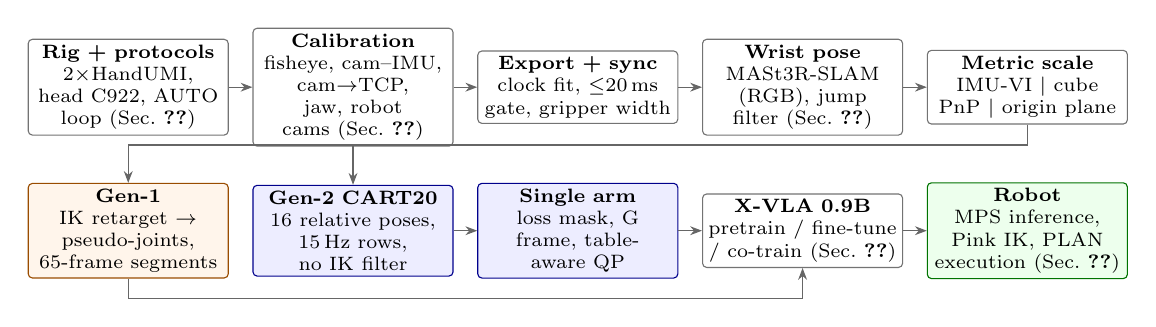
\begin{tikzpicture}[font=\scriptsize, node distance=3mm and 3mm,
  box/.style={draw=black!55, rounded corners=1.5pt, align=center, inner sep=2pt, minimum height=9mm, text width=24mm, fill=white},
  g1/.style={box, fill=orange!8, draw=orange!60!black}, g2/.style={box, fill=blue!7, draw=blue!55!black},
  dep/.style={box, fill=green!7, draw=green!45!black}, arr/.style={-{Stealth[length=1.5mm]}, draw=black!60}]
\node[box] (rig) {\textbf{Rig + protocols}\\2$\times$HandUMI, head C922, AUTO loop (Sec.~\ref{sec:hw})};
\node[box, right=of rig] (cal) {\textbf{Calibration}\\fisheye, cam--IMU, cam$\to$TCP, jaw, robot cams (Sec.~\ref{sec:cal})};
\node[box, right=of cal] (exp) {\textbf{Export + sync}\\clock fit, $\le$20\,ms gate, gripper width};
\node[box, right=of exp] (pose) {\textbf{Wrist pose}\\MASt3R-SLAM (RGB), jump filter (Sec.~\ref{sec:pose})};
\node[box, right=of pose] (scale) {\textbf{Metric scale}\\IMU-VI $\mid$ cube PnP $\mid$ origin plane};
\node[g1, below=6mm of rig] (g1) {\textbf{Gen-1}\\IK retarget $\to$ pseudo-joints, 65-frame segments};
\node[g2, right=of g1] (g2) {\textbf{Gen-2 CART20}\\16 relative poses, 15\,Hz rows, no IK filter};
\node[g2, right=of g2] (hra) {\textbf{Single arm}\\loss mask, G frame, table-aware QP};
\node[box, right=of hra] (train) {\textbf{X-VLA 0.9B}\\pretrain / fine-tune / co-train (Sec.~\ref{sec:model})};
\node[dep, right=of train] (dep) {\textbf{Robot}\\MPS inference, Pink IK, PLAN execution (Sec.~\ref{sec:deploy})};
\draw[arr] (rig)--(cal); \draw[arr] (cal)--(exp); \draw[arr] (exp)--(pose); \draw[arr] (pose)--(scale);
\draw[arr] (scale.south) |- ++(0,-2.6mm) -| (g1.north); \draw[arr] (scale.south) |- ++(0,-2.6mm) -| (g2.north);
\draw[arr] (g2)--(hra); \draw[arr] (hra)--(train); \draw[arr] (train)--(dep);
\draw[arr] (g1.south) |- ++(0,-2.5mm) -| (train.south);
\end{tikzpicture}
\caption{Pipeline. Orange: generation 1 (joint space); blue: generation 2 (Cartesian) and its single-arm variant (Sec.~\ref{sec:conv});
green: deployment. Every stage writes a manifest and is followed by a gate that accepts a unit (episode, segment, row or take) or
rejects it with a logged reason.}
\label{fig:overview}
\end{figure*}

\section{Hardware and Data Collection}\label{sec:hw}
\textbf{Attribution.} The capture device is \emph{not our design}. HandUMI was designed and published as open-source hardware by
BrikHMP18 (\url{https://github.com/murobotics-ai/handumi-hw}, Apache-2.0)~\cite{handumi_hw}, together with its software
(\url{https://github.com/murobotics-ai/handumi-sw})~\cite{handumi_sw}. The repositories were first released on 20 August 2026
under \texttt{robonet-ai}, which now redirects. We built the hardware from upstream commit \texttt{e58de33}. Our own hardware
work is limited to three modified parts, a wrist IMU added in place of the upstream VR tracking, and a fixed head camera. Our
\texttt{umihand} repository is a build copy of the upstream files plus these additions, not an original design.

\textbf{Upstream HandUMI.} HandUMI is a hand-worn variant of UMI for robot arms with parallel-jaw grippers. It mounts on the
thumb and the index and middle fingers and closes with a natural pinch; its gripper tips are detachable (AgileX Piper, ARX X5,
Dream Gripper, WidowX AI and the UMI gripper), so one body serves several robots. Upstream records wrist SE(3) from a VR
headset (PICO 4 Ultra or Meta Quest 3) and its controllers, held on the device by a printed controller support; jaw width
directly from a Feetech servo encoder rather than from fiducials or image segmentation; and wrist-view video. The finger
cradles were modelled on a 3D scan of the author's hand. The companion \texttt{handumi-sw} records, visualizes and retargets
demonstrations. Upstream has since moved to an IMX335 camera and a per-pair BOM (commit \texttt{fc7462a}); we did not adopt
that change. We forked \texttt{handumi-sw} at commit \texttt{33cc437} for an early ego-bimanual path (Quest~3S tracking,
AprilTag end-effector tracking, Feetech jaw telemetry, a reBot B601 robot profile and tracking-quality gates); none of the
demonstrations in this report were recorded with that path.

\textbf{Build.} The unit is a hand-support base with finger cradles, a fisheye camera support and a crank linkage (MR63ZZ
bearings, LM4UU linear bearings on a 4\mm shaft) that couples the finger closure to the gripper tip and to a servo read as
the jaw encoder. One unit is 12 printed parts; the package has 9 plates and 26 parts for both hands plus a generic tip, about
9\,h and 250\,g of PLA (0.20\mm layers, 2 walls, 20\% infill, Bambu X1C), about 4\,h and 110\,g per hand. A fit-check plate
(cradles and base, about 1\,h) is printed first for each hand; tight holes are fixed with $+0.05$ to $0.1$\mm XY hole
compensation, not by scaling. The tip in the package is the AgileX-Piper tip, a temporary tip for mechanism and pinch tests;
no reBot-specific tip has been designed. The upstream BOM is about US\$110 per unit.

\textbf{Sensors and our changes.} Each unit carries an Arducam 160\textdegree{} fisheye USB camera (1920$\times$1080 MJPG,
30\,fps) and a Feetech STS3215 servo read as the jaw encoder (4096 ticks/rev, polled at 100\,Hz) through a Waveshare
serial-bus adapter (CH343, 1\,Mbaud, servo id 1, which needs its 12\,V supply before the servo answers). We changed three
things. (i) VR tracking is replaced by the wrist camera plus an IMU, so the controller support is replaced by our connector.
(ii) Each unit gets an ICM-42688-P IMU on a Teensy~4.1 over SPI. The sensor has no 400\,Hz rate, so it runs at 200\,Hz
(measured 201.6 and 197.9\,Hz, each board having its own oscillator); the data-ready interrupt time-stamps each sample on the
device, packets (40-byte payload, CRC-16) go over USB CDC with a 1\,Hz status packet reporting dropped samples, and the host
fits the device-to-host clock offline so USB jitter does not enter the timeline. (iii) A fixed Logitech C922 head camera at
640$\times$480 and 30\,fps records the table and is the global view given to the policy; its autofocus is off because it
changed $f_x$ between sessions (417, 531, 501\,px). Three parts were edited in Shapr3D (Fusion~360 and FreeCAD were tried and
rejected; Fig.~\ref{fig:hwmods}): a new left controller-support connector (8 September, 85.7$\times$21.4$\times$42.1\mm,
printed twice) whose clamp plate was then lengthened by 10\mm (14 September, depth 21.4$\to$31.4\mm; 15\mm and three
$z{+}30$\mm variants were rejected), a camera mount with a second window, and a servo cover with a wider cable opening.

\textbf{Device identity.} Both Arducams report the same USB serial (\texttt{UC684}), so the recorder matches them by product
name and refuses to record unless exactly one device matches each name; IMUs are matched by Teensy USB serial and jaws by
adapter serial plus servo id, never by port order. The Teensy must be flashed as USB Serial; a RawHID build shows no port and
looks dead. One jaw crosses the encoder's 4095$\to$0 seam, so jaw normalization is circular. A 12.2\,V supply sets the servo's
``voltage'' error bit against its 12.0\,V limit; this is telemetry, not a fault. An RGB-D head camera was dropped because it
disrupted the wrist streams.

\begin{figure*}[t]
\centering
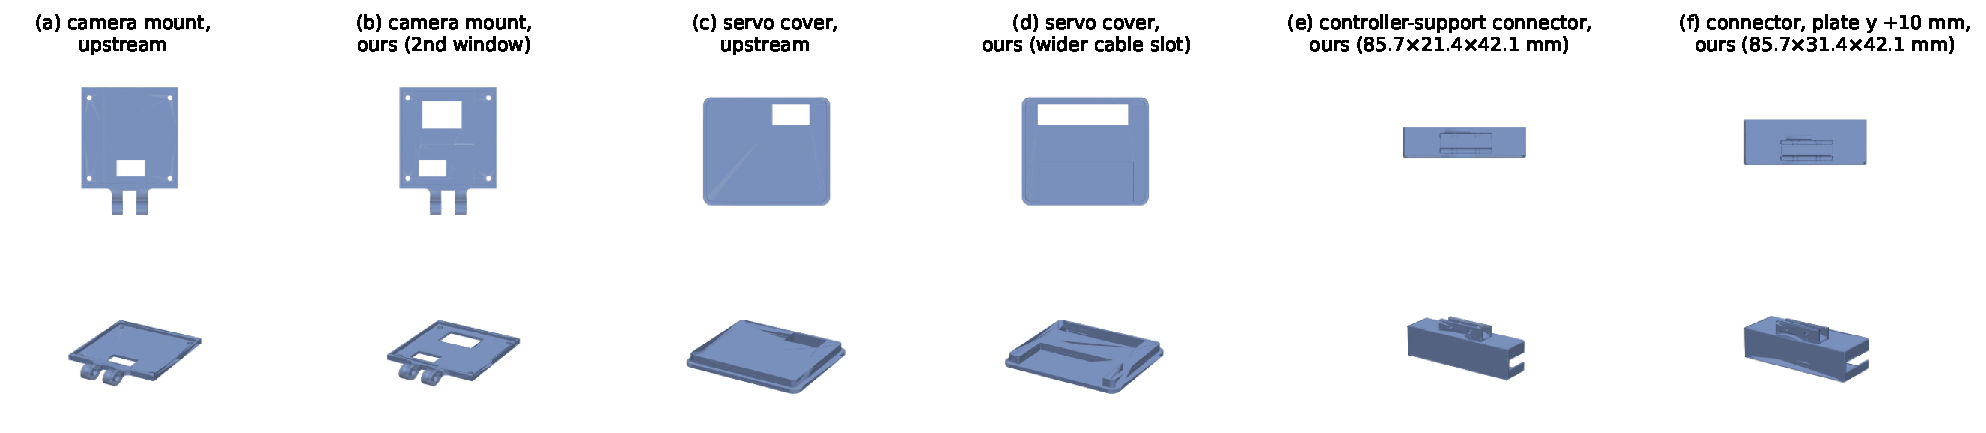
\includegraphics[width=\textwidth]{figures/fig10_handumi_mods.pdf}
\caption{Our changes to the upstream HandUMI parts (renders of the printed meshes). (a,b) camera mount: a second window cut
above the existing one; (c,d) servo controller cover: the cable opening widened; (e) the new left controller-support connector
that replaces the upstream VR-controller support; (f) its clamp plate lengthened by 10\mm, the current version.}
\label{fig:hwmods}
\end{figure*}

\textbf{Recording.} An episode directory holds one MP4 per camera, an MCAP file with IMU samples (device and host timestamps),
gripper samples (wrapped and unwrapped ticks), per-frame metadata, events and clock anchors, and metadata files; it is renamed
from \code{.incomplete} to \code{.complete} only when closed. All streams are stamped with the host monotonic clock (IMU at
receive time, gripper at the midpoint of the serial transaction, frames at capture).

\textbf{Collection protocols.} An AUTO loop (RESET $\to$ ARMING $\to$ HOLD $\to$ EPISODE $\to$ STOP) drives each take with
spoken cues. ARMING waits for stillness (in 0.25\,s windows, mean gyro magnitude below 6\textdegree/s, accelerometer-magnitude
standard deviation below 0.35\,m/s$^2$, largest sample gap below 25\,ms, for a continuous 1\,s); a hold after recording starts
gives the visual--inertial initialization window. A take that passes preliminary QA (no device or recorder error, no empty
stream, at least 25\,fps, gripper sampled at 20\,Hz or more, not frozen, within its calibrated span and travelling at least 5\%
of its range) is kept automatically.
\begin{itemize}
\item \emph{Stacking}: three 50\mm cubes (red, blue, purple) are stacked on a fixed plate in one of six orders named by the
instruction, e.g.\ ``Stack the blue cube on the bottom, purple cube in the middle, and red cube on the top, on the plate.''
Takes last 20\,s with a 10\,s reset in which the operator re-places the cubes by hand. The next order is the least-collected
one (target 50 per order), so orders are \emph{balanced}, not randomized. The layout varies through the manual reset around a
nominal layout matched to the robot workspace but was not recorded; there is no per-episode layout label.
\item \emph{Robot-like} (HRL80): 30\,s stacking takes with live feedback; wrist angular speed and acceleration on a 15\,Hz grid
are compared with the 95th percentiles of robot teleoperation data (0.996\,rad/s, 4.413\,rad/s$^2$), and a take is reviewed if
more than 10\% of ticks exceed them or fewer than two grasps occur.
\item \emph{Approach} (HRA\_red): right hand only, ``approach the red cube'', 10\,s takes.
\item \emph{Approach with origin} (HRA\_A100): as above, but each take starts with the jaw tip held on a taped origin shared with
the robot (Sec.~\ref{sec:res3}).
\end{itemize}

\textbf{Datasets.} Table~\ref{tab:data} lists every human and robot dataset used in this report. One operator recorded all human
data. The 349 stacking episodes come from 15 sessions over three days (15--17 September 2026), 2.20\,h in total (median episode
23.05\,s), per order RBP 64, RPB 62, BRP 61, BPR 56, PRB 55, PBR 51. Episodes from ten early sessions (55 episodes) are tracked as a
separate provenance domain (``early'') from the main 294 because their gripper anchors were derived afterwards; after
filtering the two domains behave alike. All robot data are teleoperated demonstrations of the same six-order stacking task on
the reBot B601.

\begin{table}[t]
\centering\footnotesize\setlength{\tabcolsep}{3pt}
\caption{Datasets. Human data were recorded with HandUMI; robot data are teleoperated reBot B601 episodes of the same stacking task.}
\label{tab:data}
\begin{tabular}{@{}lp{56mm}@{}}
\toprule
Name & Content \\
\midrule
Stacking & 349 bimanual episodes, 6 balanced orders, 15 sessions, 15--17 Sep. \\
HRL80 & 60 robot-like stacking episodes (10 per order), one session \\
HRA\_red & 200 right-hand approach takes, 3 Oct. \\
HRA\_A100 & 107 approach takes with a taped origin, 6 Oct.; 27 more on 7 Oct. \\
\midrule
R150 / R90 & 150 / 90 robot episodes (Gen-1 fine-tuning) \\
R312c & 312 robot episodes, 174{,}012 frames (Gen-2 fine-tuning) \\
R30 & episodes 150--179 of R312c, 17{,}600 frames, 5 per order \\
R384 & 384 robot episodes (scratch Gen-2 run) \\
\bottomrule
\end{tabular}
\end{table}

\section{Calibration}\label{sec:cal}
\textbf{Wrist cameras.} Kannala--Brandt (equidistant) fisheye models at full resolution, fitted with Kalibr on an 8$\times$5
checkerboard of 25\mm squares (left $f_x{=}789$, right $f_x{=}791$\,px). \textbf{Camera--IMU.} Kalibr~\cite{furgale2013kalibr}
gives time offsets of 30.2 and 32.8\,ms with mean reprojection errors of 6.0 and 5.6\,px, which is high and one reason pose
accuracy is validated separately (Sec.~\ref{sec:pose}).

\textbf{Camera to TCP.} The TCP is the pinch centre with $x$ along the approach direction, $y$ along jaw closing and $z=x\times y$.
The rotation is a fixed axis permutation ($x_\text{TCP}=z_\text{cam}$, $y_\text{TCP}=-x_\text{cam}$, $z_\text{TCP}=-y_\text{cam}$);
the translation comes from caliper measurements (95\mm forward, 95\mm down) rotated by the camera pitch measured from IMU gravity
(20.7\textdegree), giving $t=[0, 55.3, 122.5]$\mm, consistent to about 1\mm with a cube-based fit. Following UMI's use of a CAD
constant, it was measured on one unit and applied to both.

\textbf{Gripper width.} Each frame takes the nearest gripper sample. The recorded normalized value was unreliable (the open end
lay beyond the mechanical stop and the left direction flipped between sessions), so Gen-1 recomputes width from raw ticks with
a per-episode closed anchor and the device span (1136.6 / 1248.2 ticks), width $=\mathrm{clip}(f,0,1)\times 67.5$\mm (aperture
$67.5\pm5$\mm, estimated from video of 50\mm-cube grasps). Gen-2 uses a later caliper calibration (gcal1): piecewise-linear
knots at 0/20/40/60/80\mm, normalized as $g=\mathrm{clip}(w/80\,\text{mm},0,1)$, 0 = closed.

\textbf{Clocks and synchronization.} IMU device time is mapped to host time by a least-squares slope with the intercept
re-anchored at the 5th percentile of the residuals, because USB latency only ever adds delay; the camera--IMU offset is then
applied. Cameras free-run at slightly different rates (30.003--30.026\,Hz), so frames are paired by nearest capture time. For
bimanual data the left wrist is the master clock; a row is valid if both wrist poses are valid and the right wrist and head
frames are matched within 20\,ms.

\textbf{Robot side} (single-arm work). The robot's fixed head C922 (the same camera and position as during HRA\_red) was calibrated
on the same checkerboard (48 frames, RMS 1.05\,px, $f=728.7$\,px), and its pose in the robot base was found by touching four board
corners with the right jaw tip (Kabsch alignment of FK positions and board PnP; residuals 2--6\mm). The robot wrist camera is
calibrated from 13 board views (0.16\,px RMS, $f=651.4$\,px), and its hand-eye transform is solved with four methods (including
Tsai--Lenz~\cite{tsai1989handeye}) that agree to 1--2\mm and 0.3\textdegree{} in board-in-base pose. The camera sits 169.5\mm
behind the TCP and 76\mm off its axis, and its optical axis points 33\textdegree{} below the TCP $x$ axis.

\textbf{TCP is not the jaw tip.} The IK stack's TCP lies about 82\mm ahead of the physical jaw tip along the TCP $x$ axis (found by
projecting FK points into the wrist image). Contact is therefore modelled by the URDF fingertip box (70--80\mm behind the TCP,
$\pm$19.6\mm), whose lowest corner counts as contact.

\section{Wrist Pose and Metric Scale}\label{sec:pose}
\textbf{Monocular pose.} UMI localizes all demonstrations in one ORB-SLAM3 map per scene. On our data this failed: maps built
before a scene change did not relocalize, and on the marker benchmark below its position tracks reversed direction often
(median reversal rate 0.24 versus 0.07 for the method we adopt). We run MASt3R-SLAM~\cite{murai2025mast3rslam}
(official code, pinned commit, a build fix only) on the RGB wrist video undistorted to a pinhole view, single-threaded, every
frame, fixed seed. After global optimization every frame is re-expressed on its final keyframe,
\begin{equation}
T_{WC}(f) = T_{WK}^{\text{final}}(k)\,T_{WK}^{\text{track}}(k)^{-1}\,T_{WC}^{\text{track}}(f),
\end{equation}
a Sim(3) chain; frames tracked during relocalization are invalid unless they later became keyframes. Fig.~\ref{fig:traj} shows
typical trajectories.

\begin{figure*}[t]
\centering
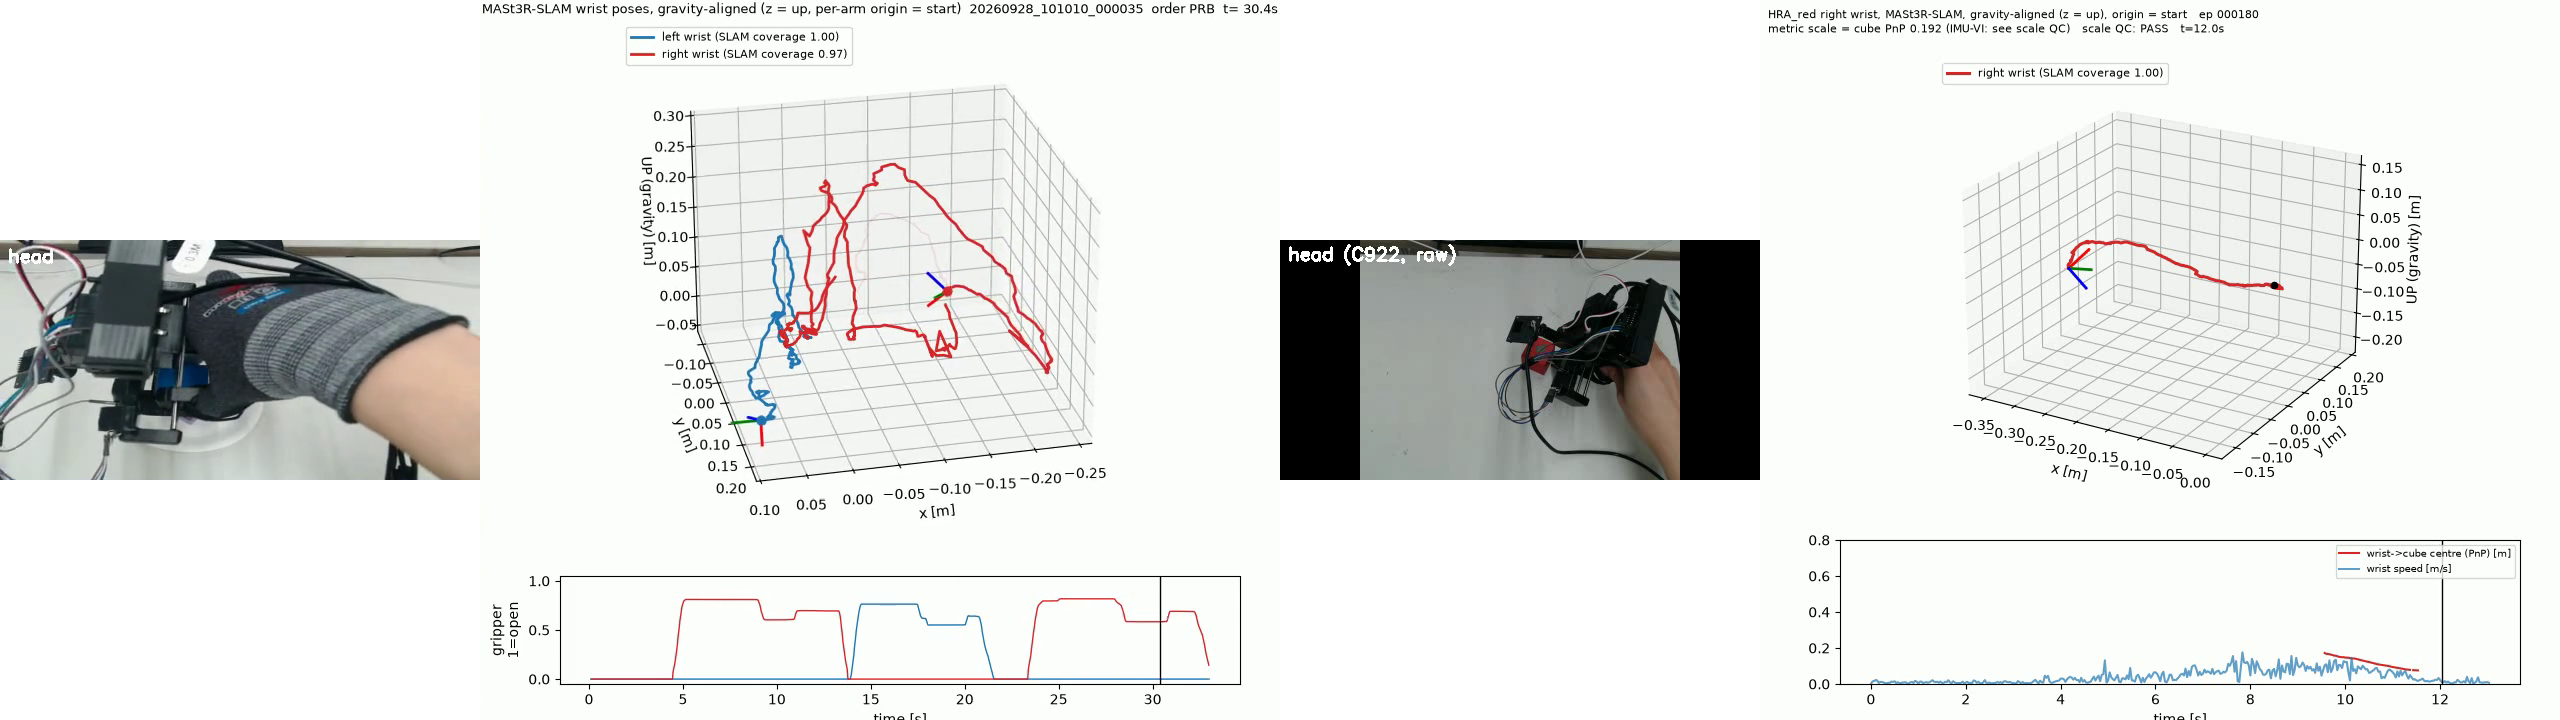
\includegraphics[width=0.8\textwidth]{figures/fig7_mast3r_trajectories.png}
\caption{MASt3R-SLAM wrist trajectories of an HRL80 stacking take (order PRB). Left: head camera and both wrist fisheye
cameras. Right: trajectories gravity-aligned (z up), each arm's origin at its start pose, current tool axes drawn (x red,
y green, z blue), metric scale from the IMU; below, both grippers (1 = open). Videos of three takes (PRB, RBP, PBR):
\texttt{docs/media/mast3r\_trajectories/hrl80\_0000\{35,55,60\}\_wrist.mp4} in the repository.}
\label{fig:traj}
\end{figure*}

\textbf{Scale 1: IMU visual--inertial.} The SLAM trajectory is metric up to a per-episode scale $s$. With $R_{wb}=R_{wc}R_{cb}$,
accelerometer samples $f_b$ box-averaged around each frame, and the camera and lever-arm accelerations $a_\text{cam}$,
$a_\text{lever}$ obtained as Savitzky--Golay second derivatives (order 3, window $W$) of the SLAM camera position and of
$R_{wc}t_{cb}$, each frame contributes three rows of
\begin{equation}
R_{wb}\,f_b - a_\text{lever} = s\,a_\text{cam} - g,
\end{equation}
solved for $s$ and $g\in\mathbb{R}^3$ by Huber-weighted iteratively reweighted least squares over the longest valid run. Both
sides pass the same filter, so nothing is integrated twice. A scale is valid if $s>0$ and $|g|\in[8.81,10.81]$\,m/s$^2$.

\textbf{Pose benchmark.} 14 demonstrations (28 hand tracks) with four 80\mm ArUco markers in view, run on the same GPU as the
dataset; ground-truth scale is the median ratio of marker to SLAM displacement over frame pairs ten frames apart. $W=15$ without
bias was selected on a fit split of 9 demonstrations; on the 5 held-out demonstrations (10 tracks) MASt3R-SLAM with IMU scale
gives median tracking coverage 1.00 versus 0.03 for ORB-SLAM3 with a stored map, scale error p50/p90 of 4.6/17.0\% (versus 18.5/23.8\% for one global constant), rotation
error p50/p90 0.84/2.13\textdegree{} and a UMI-style 16-step relative position error p90 of 11.3\mm. The demonstrations themselves
have no ground truth.

\textbf{Scale 2: a cube of known size.} For slow, smooth motions the accelerometer barely constrains the IMU fit: across the 200
HRA\_red takes the IMU scale has a median of 0.012 and is zero or negative, which is physically impossible, in 95 of them
(Fig.~\ref{fig:cube}b). The red cube (edge 38\mm) is static. In frames where it is visible we segment it in HSV, fit its
silhouette with two- or three-face models, or a single-face model within 35\textdegree{} of head-on, and solve PnP. Since the
cube's centre $c_i=p_i + k\,R_i t_i$ must be constant, the inverse scale follows in closed form,
\begin{equation}
k = -\frac{\sum_i (p_i-\bar p)\cdot(u_i-\bar u)}{\sum_i\lVert u_i-\bar u\rVert^2},\qquad u_i=R_i t_i,\quad s=1/k,
\end{equation}
with MAD trimming and 200 bootstrap resamples. A take needs at least 10 PnP frames, a bootstrap spread of at most 10\% and a
cube-centre residual of at most 2\,cm. On the HRL80 stacking takes, where the IMU scale is reliable, 37 of 57 right-hand episodes
are PnP-valid and the PnP/IMU ratio has a median of 1.062 (p16--p84 0.959--1.274; Fig.~\ref{fig:cube}a).

\begin{figure*}[t]
\centering
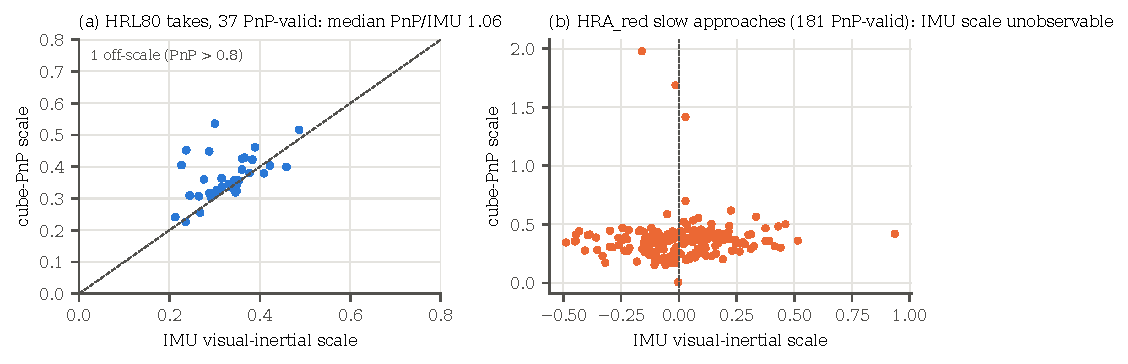
\includegraphics[width=\textwidth]{figures/fig6_cube_scale.pdf}
\caption{Per-episode metric scale of the MASt3R-SLAM trajectory from the IMU and from cube PnP. (a) HRL80 stacking takes,
where the IMU scale is reliable. (b) HRA\_red approach takes: the IMU scale scatters around zero.}
\label{fig:cube}
\end{figure*}

\textbf{Scale 3: the table plane at a shared origin.} In HRA\_A100 the fingertip touches the plate during the origin hold, so the
first MASt3R keyframe sees the table at a known distance. Excluding the finger, up to three planes are fitted by RANSAC and the
largest one parallel to the plate is taken as the table; $s=|n\cdot t_\text{tip}|/(s_0\,|d|)$ with $t_\text{tip}$ the fingertip in
camera coordinates and $s_0$ the keyframe's Sim(3) scale. Against cube PnP on 40 takes the ratio has a median of 0.999 and a
per-episode error of p50 8\%, p90 37\%. Each episode uses cube PnP where it is valid and the plane otherwise (35 and 72 of 107);
the IMU is not used.

\textbf{Silent pose jumps.} Comparing ego and robot state statistics showed per-row state jumps above 100\mm in the ego data that
the robot data does not have. Two causes were mixed. First, an exported dataset contains only training rows, so ``adjacent''
frames can be seconds apart: 1{,}482 of the 2{,}598 apparent jumps above 30\mm (57\%) are such time gaps, and adjacency has to be
decided from row timestamps. Second, the remaining jumps are real: MASt3R-SLAM occasionally moves the camera by 10\,cm or more
within one 30\,Hz frame without flagging tracking loss (55 raw steps faster than 3\,m/s in 24 training episodes, none preceded by
a loss flag). The filter flags a step above 100\mm or 45\textdegree{} per 66.7\,ms row, or an isolated step above 50\mm between two
steps slower than 0.3\,m/s. If the pose returns, the event is a spike and only its samples are invalidated; otherwise it is one-way
and the rest of that arm's track is dropped, because a start-anchored state would be wrong from then on.

\textbf{Camera--IMU consistency.} Sessions whose gyro and SLAM angular velocities disagree (median cosine near 0 against
0.92--0.98 elsewhere) are quarantined. For the approach data, the exported camera--IMU rotation of the right wrist turned out to be
wrong by about 18\textdegree{} about the camera $x$ axis (cube-axis error 17.8$\to$3.4\textdegree{} after correction); IMU tilt
statistics computed before the correction are wrong by up to that amount, while training poses whose scale comes from cube PnP
were unaffected.

\section{Converting Human Motion into Robot Data}\label{sec:conv}
\subsection{Generation 1: joint-space retargeting}
\textbf{Segments and gates.} Synchronized valid rows are cut into non-overlapping 65-frame segments (2.17\,s). Per arm, a segment
needs a valid metric scale, at least 95\% of rows inside the robot workspace (a target is inside if its nearest neighbour among
6{,}000 robot teleoperation TCP poses is within 50\mm and within 20\textdegree{} in orientation), and an IK solution on every row.
A segment is bimanual if both arms pass. Each TCP trajectory is mapped to a reBot B601 6-DoF arm by least-squares IK on its URDF.
Absolute workspace geometry is not recoverable across episodes, so each segment is re-anchored at one fixed robot start pose (the
median active pose of our robot teleoperation data); motion is transferred, absolute cube positions are not. The jaw encoder
becomes a binary gripper command.

\textbf{Funnel.} Table~\ref{tab:funnel} lists what each gate removes. 65 episodes fail the $\le$20\,ms synchronization requirement
for a full 65-frame window; the remaining 284 yield 1{,}306 candidate bimanual segments, of which 677 leave the robot workspace,
50 fail the metric-scale check and 18 fail IK, leaving 561 (43.0\%). Two sessions (6 episodes) were quarantined for an
IMU--camera rotation inconsistency; none contributed a segment. 47\% of segments start in the first 5\,s of an episode.

\textbf{Split.} The 259 episodes with at least one bimanual segment are split at random by episode (seed 0, 10\%): 233 train / 26
val, i.e.\ 504/57 segments and 32{,}760/3{,}705 frames. No episode spans both sides. The split is not stratified; validation has
3--6 episodes per order, 22 main / 4 early, from 9 of the 13 non-quarantined sessions.

\begin{table}[t]
\centering\footnotesize
\caption{Gen-1 processing funnel for the 349 stacking episodes (counts recomputed from the census files in the repository).}
\label{tab:funnel}
\setlength{\tabcolsep}{4pt}\begin{tabular}{@{}lrr@{}}
\toprule
Stage & Episodes & Segments \\
\midrule
Recorded (KEEP) & 349 & -- \\
Pose + gripper exported (698 tracks) & 349 & -- \\
Sync $\le$20\,ms, $\ge$65-frame window & 284 & 1{,}306 \\
\quad $-$ workspace / metric scale / IK & & $-$677 / $-$50 / $-$18 \\
$\ge$1 bimanual segment (training pool) & 259 & 561 \\
\quad train / val (by episode, seed 0) & 233 / 26 & 504 / 57 \\
\bottomrule
\end{tabular}
\end{table}

\textbf{Retargeting v2.} The single start anchor was the main source of loss: every segment began at one robot posture, so most
left the workspace and the retargeted trajectories covered one posture cluster. v2 replaces it with multi-seed retargeting under a
strict budget: every real-robot quantity (seed bank, workspace gate, posture penalty, trajectory windows) comes from 30 robot
episodes only, and results are measured against a disjoint set of 120 robot episodes. A seed bank of $2^{17}$ Sobol samples is
filtered by workspace, table floor, manipulability and inter-arm clearance ($\ge$75\mm), leaving 1{,}195 seeds. Variant K rolls out
the best 8 seeds under a cost on position, rotation, joint velocity and acceleration; Kr adds a posture distance to robot data;
trajectory-window retrieval (TR) starts each human segment from the closest feasible robot trajectory window (64 nearest by a 96-D
relative-motion feature). Table~\ref{tab:retarget} compares them on the same 1{,}229 candidate segments. TR is the most robot-like:
posture distance to the held-out robot data falls from 1.49 to 0.27\,rad (median) and start postures span 100 clusters instead of 1.
It solves fewer segments than the kinematic variants because it cannot place fast motions; among the 686 segments both TR and Kr
solve, their joint-velocity distributions are similar (W1 0.00207 vs 0.00226), so the posture gain, not a dynamics gain, is what TR
adds. The remaining failures are almost all ``no workspace-compatible window'' (399 of 402 unsolved).

\begin{table}[t]
\centering\footnotesize\setlength{\tabcolsep}{3.5pt}
\caption{Retargeting variants on the 1{,}229 candidate segments of the 259 episodes, measured against 120 held-out robot
episodes. NN: nearest-neighbour joint-space distance to robot postures (rad, p50/p90); W1: Wasserstein distance of
$|\Delta q|$ per step.}
\label{tab:retarget}
\begin{tabular}{@{}lcccc@{}}
\toprule
Variant & Usable & NN p50 / p90 & Start clusters & W1 $|\Delta q|$ \\
\midrule
v1 single anchor & 36.5\% & 1.49 / 1.55 & 1 & 0.00197 \\
v2-K multi-seed IK & 66.6\% & 1.21 / 1.60 & -- & 0.00275 \\
v2-Kr + posture penalty & 67.0\% & 0.44 / 0.74 & -- & 0.00310 \\
v2-TR window retrieval & 56.1\% & 0.27 / 0.45 & 100 & 0.00208 \\
\bottomrule
\end{tabular}
\end{table}

\textbf{Robot-like re-collection.} To test whether the loss is a collection-style problem we recorded HRL80 (60 episodes, 10 per
order) with the robot-like protocol; its interpretation rules were fixed before retargeting. Live rotation speed halved (median
over-threshold fraction 0.144 to 0.067), but the per-episode TR yield did not change (0.59 vs 0.59) and TR usable rose only from
56.1\% to 58.9\%; the per-episode correlation between live robot-likeness and TR yield is weak (Spearman $\rho=-0.11$, $p=0.05$,
pooled $n=316$). Workspace placement, not collection style, remains the main failure. The final TR dataset combines both
collections: 996 segments (896 train / 100 val) from 316 source episodes, with the original 689 segments preserved bit-identically.

\subsection{Generation 2: the Cartesian contract (CART20)}
Retargeting to robot joints had two costs: the workspace and IK gates removed a third to a half of the candidate motion, and the
joint-space target differed from the Cartesian action space our robot policies are fine-tuned in. Gen-2 converts each human wrist
trajectory directly into the relative end-effector representation of the robot teleoperation data, so that ego and robot samples
share one tensor contract.

\textbf{Contract.} Rows are stored at 15\,Hz. For row time $t$ and each arm the action is a chunk of 16 future poses
\begin{equation}
A_k = T(t)^{-1}\,T(t+k\Delta),\qquad k=1,\dots,16,
\end{equation}
with $\Delta = 50.05$\,ms (the robot data's step, 0.80\,s in total), current-anchored rather than sequential, and interpolated on
the raw 30\,Hz track (linear in position, SLERP in rotation, only between valid samples no more than 50\,ms apart). Each arm
contributes position, a 6-D rotation and a gripper value (20 dimensions for two arms, ``CART20''); the model's 32-D action is padded
with 12 dimensions that are exactly zero and never supervised. The state is each arm's pose relative to its own task-start pose,
$T(t_0)^{-1}T(t)$, plus both gripper values, the same layout as the robot state (there is no shared left--right SLAM frame). The
gripper is the jaw aperture divided by 80\mm; the largest observed value is 0.847, so ``fully open'' is never reached. A row is
kept only if both arms are valid at $t$, all 16 targets are valid and a head-camera frame exists within 20\,ms; there is no padding
and no workspace or IK selection. Eleven synthetic tests pin the contract.

\textbf{Data.} The source is the 273 original stacking episodes with valid per-hand IMU scale and 60 HRL80 episodes, of which 3
are refused because one hand's IMU scale is invalid, leaving 330. Of 111{,}533 rows, 57{,}283 (51.4\%) are usable; the rest fall on
tracking losses, synchronization gaps or the last 0.8\,s of an episode. The split is frozen from Gen-1 (validation = the 26 held-out
episodes plus HRL80 episodes 49--54): 298 train episodes with 51{,}612 rows and 32 validation episodes with 5{,}671 rows. The
pose-jump filter (Sec.~\ref{sec:pose}) acts on 44 events in 42 training episodes and removes one episode entirely; training
shrinks to 297 episodes and 48{,}411 rows ($-6.20$\%), validation is unchanged. The largest step between time-adjacent rows falls
from 422.5 to 90.5\mm and steps above 100\mm from 18 to 0; 7 raw steps faster than 3\,m/s remain inside valid rows.

\textbf{How ego data differs from robot data.} On 60 ego and 60 robot episodes, with ego poses attached to a robot start pose: the
robot's IK reaches 99.7\% (left) and 99.5\% (right) of ego positions, and 72.3\%/74.6\% of full ego poses. The IK configuration used on
the robot, which locks one wrist joint, reproduces only 45.2\%/52.2\% of the robot's \emph{own} recorded poses, a deployment
limitation that exists without any human data. Ego hands use a smaller workspace (state p95 0.221/0.214\,m versus 0.395/0.369\,m)
with similar 0.4\,s translations (p95 93/99 versus 91/100\mm), and both ego hands are still at the same time far more often (19.5\%
versus 2.4\% of samples). The largest difference is visual: the variance of the image Laplacian, a sharpness measure, has a median
of 1{,}854/1{,}487 for the ego wrist fisheye views and 59/64 for the robot's wrist cameras.

\textbf{Robot-like wrist rendering.} To narrow the visual gap, a fisheye frame can be re-rendered as a virtual pinhole camera with
the same orientation, so labels stay valid: horizontal field of view 62--70\textdegree, principal point shifted down so that the
jaws sit low as on the robot, then downscaled, blurred, JPEG-compressed and photometrically jittered. ROBOT100 applies this to every
frame.

\subsection{Single-arm variant and a shared task frame}
\textbf{Right-only contract.} The tensor layout is unchanged: the left state is the identity pose with gripper 0, the left action is
zero motion, and a 20-D loss mask supervises only the right arm's position and rotation (9 dimensions; the jaw is unused). The task
string is ``Approach to the red cube''.

\textbf{Robot-camera rendering (robotcam v2).} The first version (v1) rendered the wrist view with the guessed camera above. The
measured robot C922 has a 52\textdegree{} horizontal field of view with a centred principal point, so v1 showed the cube much later
in the approach than the robot camera does. In v2 every robot-camera pixel's ray is projected into the fisheye model and resampled,
and labels are expressed as robot-TCP poses through the hand-eye transform (robot TCP $\to$ UMI TCP: $-33$\textdegree{} about $y$,
$t=(-94.8, 2.4, 38.4)$\mm).

\textbf{Task frame G.} A cross of tape on the head-camera base plate, about 35\,cm from the robot gripper, is the task origin. The
robot's right jaw tip touched three points on the tape line; they are collinear to within 0.38\mm over a 60.4\mm baseline and agree
in height within 2\mm. G has its origin at the cross centre, $x$ along the tape towards the human side and $z$ along base $z$:
origin $(59.0, -74.9, 6.2)$\mm in the robot base, heading 47.09\textdegree. With the 35\mm plate the table is at $z=-27.1$\mm. On the
human side the origin pose is the median position and mean rotation over the origin hold; its yaw is measured per take by matching
table features around the cross against a reference take (error p50 0.21\textdegree, p90 1.17\textdegree), with tilt from IMU
gravity. Assuming a mean yaw instead had produced false rejections and a 57\mm endpoint-height spread (35\mm with measured yaw). The
hold itself repeats to 14\mm (p50; p90 37\mm) and 6.2\textdegree{} (p50), with the camera pitched 63.7\textdegree{} down.

\textbf{Table-aware conversion.} Expressing human motion in G and starting it from a robot start pose can push the fingertip into the
table. The trajectory is therefore warped from its own start towards the robot start pose with smoothstep weights that decay to
zero over the take, on separate schedules for horizontal position, height and rotation, so the human endpoint near the cube is kept.
A height correction $c$ is then solved per take as a quadratic program,
\begin{equation}
\begin{aligned}
\min_c\;& \textstyle\sum c^2+50(\Delta c)^2+2000(\Delta^2 c)^2+60\,m\,(c-g)^2\\
\text{s.t.}\;& z_\text{tip}+c\ge z_\text{table}+5\,\text{mm},
\end{aligned}
\end{equation}
with $c_0=0$, an endpoint lift of at most 30\mm and $g$ pulling low frames towards 12\mm clearance; the result is replayed through
IK. Takes are classed PASS (lift $\le$20\mm), PASS-CORRECTED (20--30\mm) or rejected (IK success below 98\%, missing origin hold or
yaw, hold moved more than 10\mm). Table~\ref{tab:ct} shows the variants. CT4 decays position, height and rotation on separate
schedules; CT5 adds measured origin yaw, the corrected IMU gravity, absolute state in G and the hold gate; CT6 moves the robot start
6\,cm back and 4\,cm down. CT5 and CT6 keep 86 takes with fingertip clearance p50 12.6\mm and minimum 7.6\mm; most rejections are the
first session (before the origin hold existed) or takes whose origin yaw could not be measured.

\begin{table}[t]
\centering\footnotesize\setlength{\tabcolsep}{3pt}
\caption{Table-aware conversions of HRA\_A100. Accepted = PASS + PASS-CORRECTED. Clearance: fingertip above the table after
correction, accepted takes.}
\label{tab:ct}
\resizebox{\columnwidth}{!}{\begin{tabular}{@{}lcccc@{}}
\toprule
Variant & Takes & Accepted & Main rejections & Clearance p50 / min \\
\midrule
C (mean yaw) & 107 & 81 & lift $>$30\,mm 10, old 7 & 19.5 / 7.0\mm \\
CT4 (per-axis decay) & 107 & 87 & lift 10, old 7 & 20.6 / 7.9\mm \\
CT5 (yaw, G, hold gate) & 107 & 86 & yaw not measured 9, old 7 & 12.6 / 7.6\mm \\
CT6 (start back/down) & 107 & 86 & as CT5 & 12.6 / 7.6\mm \\
CT7 (low start, +27) & 134 & 90 & IK 19, yaw 11, old 7 & 12.4 / 7.6\mm \\
\bottomrule
\end{tabular}}
\end{table}

\section{Model and Training}\label{sec:model}
\textbf{Model.} X-VLA~\cite{zheng2025xvla} through LeRobot~\cite{cadene2024lerobot}, from the public \texttt{xvla-base} checkpoint:
a Florence-2~\cite{xiao2024florence2} vision-language encoder, a 24-layer soft-prompted transformer (hidden 1024, 16 heads) and a
flow-matching~\cite{lipman2023flow} action head; 879M parameters, all trainable. Inputs are the three views (head, left wrist, right
wrist, resized to 224\,px), the instruction and the proprioceptive state. Training draws $t$, forms $x_t=\varepsilon t+a(1-t)$ and
regresses the clean action; inference integrates from noise in 10 steps by default. For Gen-2 the public head (20-D action and
state) was widened to a 32-D action and 20-D state, with existing rows copied exactly and the widened model checked to reproduce the
base.

\textbf{Which soft prompt?} X-VLA conditions on a dataset/embodiment id that selects one of 30 sets of 32 soft prompts and
domain-specific state/action projections. Our first runs used id~0. Reading the public base weights shows that only slots 10--17
were ever trained: in the other 22 slots the encoder and decoder biases are exactly zero and the prompt weights stay near their
initialization. Ids 0 and 6, both used by us, were therefore untrained slots. The trained slots are not a better start either: the
initial loss on R312c is 1.11 for slot 0, 1.12 for 6, 1.61 for 15, 2.35 for 10, 2.65 for 16, 4.07 for 17 and 22.80 for 11. All
Gen-2 runs use the unused slot 20 as our embodiment's own slot.

\textbf{Gen-1 recipe.} For state time $t$ the model predicts a 30-step chunk $a_i = q_{t+5+i}-q_t$, $i=0,\dots,29$, of cumulative
joint displacements of the retargeted pseudo-joints (a 5-frame lead, so the chunk covers 0.2--1.17\,s ahead), plus the absolute
gripper. The state is 14-D (6 joint angles and a binary gripper per arm). Two auxiliary terms tie joint space to the measured human
motion: (C) the relative TCP position of the measured trajectory in spare action dimensions (weight 2.0) and (D) a forward-kinematics
loss between $\mathrm{FK}(q_t+\hat a_i)$ and the measured TCP position (weight 20). Targets are measured human transitions, never
relabelled robot commands. Optimization: 300k steps, batch 4, AdamW (lr $10^{-4}$, the vision-language group at 0.1$\times$, weight
decay $10^{-4}$, 1k warm-up, cosine decay to $2.5\times10^{-6}$), gradient clipping 10, fp32, one RTX~4090, a checkpoint every 10k.
The checkpoint selection rule (minimum geo score, Sec.~\ref{sec:eval}) was fixed before training.

\textbf{Gen-2 recipe.} MSE on action dimensions 0--19 only; dimensions 20--31 are zeroed at the transformer's input and output at
every denoising step, in training and at inference, and a preflight checks that padding targets are ignored and padding gradients
vanish. Batch 8, 8-bit AdamW (policy learning rate $10^{-4}$, warm-up 1k, cosine decay ending exactly at the last step), bf16 mixed
precision, seed 1000. For the single-arm data, masked targets are replaced by the detached prediction before subtraction and the loss
is normalized by the number of supervised elements; a 300-step smoke test verified that masked and padded dimensions receive exactly
zero gradient. Fine-tuning starts a fresh optimizer and uses the robot dataset's normalization statistics; co-training draws exactly
four ego and four robot samples per batch.

\textbf{Operations.} Jobs run on a Ray cluster pinned to an RTX~4090 or RTX~5090 node (their PyTorch versions differ, so cross-node
runs are not bit-identical). Launchers refuse to start on a busy GPU, a code-hash or domain-id mismatch, a failed gripper-contract
gate or low disk space; a short smoke run with save and resume precedes each main run; and an archiver copies every checkpoint to
external storage with SHA-256 verification before deleting it from the node.

\section{Evaluation Protocol}\label{sec:eval}
\textbf{Gen-1 offline.} On the 26 held-out episodes we take 7 start frames from each of the 57 validation segments (every 5 frames in
0--30), giving 399 samples and 798 arm-samples, and compare the predicted chunk with the recorded future. For horizons
$k\in\{1,4,8,16,30\}$ we report the TCP position error between $\mathrm{FK}(q_t+\hat a_k)$ and the measured TCP (median, mm), the
joint MAE and that of a \emph{zero-motion} predictor ($\hat a\equiv0$), and the cosine between predicted and measured TCP
displacement. The \emph{geo score} is the mean of the median TCP error over the five horizons. Because most samples are
near-static, every metric is also reported on the \emph{moving} subset, arm-samples whose measured TCP moves $\ge$20\mm by $k{=}30$
(187 of 798, 23.4\%). This gate was added after the 60k checkpoint had been evaluated and is used for reporting only.

\textbf{Prompt swap.} To test instruction use, the final checkpoint is queried on every sample with each of the six order
instructions under one noise seed, and with the true instruction under two further seeds. The spread of the six predictions
measures the instruction's effect; the spread across seeds is the sampling-noise floor. \textbf{Paired bootstrap}: episode-level
resampling (10k draws, identical for both models) of the relative difference in geo score between two initializations.

\textbf{Gen-2 diagnostics.} Teacher-forced direction cosine on robot frames (predicted versus recorded translation at $k$=4/8/16 for
moving frames), repeated under all left/right swaps and axis sign flips; an image/state domain swap; optical-flow versus pose-axis
correlation of the wrist videos as a convention check; wrist sharpness as the variance of the Laplacian; training-loss comparisons
as window means and ratios; and, for the single-arm data, held-out loss (the masked training loss on all validation rows).

\textbf{What the splits do not test.} Validation episodes share operator, scene, sessions and all six orders with training, and
layouts are unlabelled. Results therefore measure within-distribution generalization to new \emph{episodes}, not to new layouts,
orders or scenes. Every number in this report is recomputed from evidence files in the repository by a claim-verification script.

\section{Results: Joint-Space Stacking (Gen-1)}\label{sec:res1}
\begin{table*}[t]
\centering\footnotesize
\setlength{\tabcolsep}{7pt}
\caption{Gen-1 offline held-out results (26 episodes). TCP error: median FK position error (mm); MAE: joint MAE (deg), with the
zero-motion predictor in parentheses; cos: TCP direction cosine. 160k is the pre-registered selection, 300k the final step.}
\label{tab:results}
\begin{tabular}{@{}llccccc@{}}
\toprule
 & & \multicolumn{5}{c}{horizon $k$ (steps of 1/30\,s after a 5-frame lead)} \\
\cmidrule(l){3-7}
Subset & Metric & 1 & 4 & 8 & 16 & 30 \\
\midrule
\multirow{3}{*}{All (798)} & TCP err., 160k & 1.3 & 1.7 & 2.2 & 3.1 & 5.7 \\
 & TCP err., 300k & 1.5 & 1.8 & 2.2 & 3.2 & 5.7 \\
 & MAE, 300k & 0.30 (0.15) & 0.34 (0.19) & 0.42 (0.25) & 0.57 (0.36) & 0.97 (0.51) \\
\midrule
\multirow{4}{*}{Moving (187)} & TCP err., 160k & 11.2 & 15.0 & 19.9 & 29.2 & 39.1 \\
 & TCP err., 300k & 11.2 & 15.0 & 19.4 & 29.3 & 39.9 \\
 & MAE, 300k & 2.02 (2.32) & 2.68 (3.36) & 3.29 (4.38) & 4.30 (6.34) & 6.59 (8.68) \\
 & cos, 300k & 0.72 & 0.80 & 0.84 & 0.86 & 0.90 \\
\bottomrule
\end{tabular}
\end{table*}

Table~\ref{tab:results} and Fig.~\ref{fig:eval} summarize the evaluation of the model fine-tuned on the 561 Gen-1 segments.

\textbf{(1) Aggregate errors mostly reflect static phases.} The geo score reaches 2.78\mm at 160k and 2.88\mm at 300k and is flat
after about 120k (Fig.~\ref{fig:eval}a). On moving samples the error is an order of magnitude larger: 11\mm at the shortest horizon
and 40\mm at $k{=}30$, with a p90 of 90\mm; the moving-subset geo score is 23.0\mm versus 2.9\mm on all samples.

\textbf{(2) On moving samples the policy predicts the direction of motion and beats a no-motion baseline.} The direction cosine
rises from 0.72 at $k{=}1$ to 0.90 at $k{=}30$, and joint MAE is 13--32\% lower than the zero-motion predictor across horizons
(6.59 versus 8.68\textdegree{} at $k{=}30$; Fig.~\ref{fig:eval}b).

\textbf{(3) On all samples, the policy is worse than predicting no motion.} Joint MAE is about twice the zero-motion MAE at every
horizon (0.30 versus 0.15\textdegree{} at $k{=}1$): during static phases the policy predicts small spurious motion, and the median
predicted-to-measured displacement ratio is 1.41 at $k{=}1$. On a robot this would appear as creep before grasps or after
placement; residual pose noise in near-static windows is a plausible, untested contributor. At $k{=}30$ the spread of predictions is
0.77 of the spread of targets, so the long horizon is under-dispersed rather than collapsed, and fast or unusual motions are pulled
towards the mean.

\textbf{(4) The order instruction changes predictions but does not improve them.} In the prompt swap (Fig.~\ref{fig:eval}c), the six
instructions move the predicted TCP by a median of 4.8\mm at $k{=}30$ on moving samples, about 50$\times$ the sampling-noise spread
(0.09\mm) but only 8\% of the predicted displacement (62\mm). The true instruction is not closer to the recorded motion than the
wrong ones: its error is 39.9\mm versus 39.5\mm for the mean wrong instruction, and its mean rank among the six is 3.55 (chance 3.5;
rank 1 in 16\% of cases, chance 17\%), with the same picture at every horizon and on all samples. The prediction with the true
instruction and the original seed reproduces the reference evaluation to within $10^{-5}$\mm. Much of a 2.2\,s segment is
order-independent (reaching, lifting), and once stacking has begun the order is partly visible in the scene, so nothing in training
forces the model to use the instruction; a test restricted to choice points needs more samples than 26 validation episodes provide.
Per-order breakdowns (3--6 validation episodes per order) are too small to rank orders.

\begin{figure*}[t]
\centering
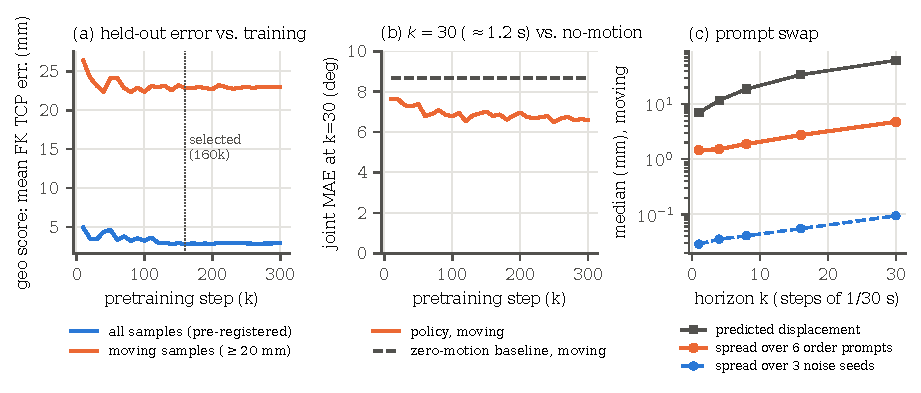
\includegraphics[width=\textwidth]{figures/fig4_eval.pdf}
\caption{Gen-1 offline evaluation. (a) Geo score over training on all versus moving held-out samples; the pre-registered rule
selects 160k. (b) Joint MAE at $k{=}30$ on moving samples, policy versus zero-motion predictor. (c) Prompt swap on the final
checkpoint: prediction spread across the six order instructions (same seed) versus across three noise seeds (true instruction).}
\label{fig:eval}
\end{figure*}

\textbf{Data lost before learning.} 57\% of the candidate segments are removed; the workspace gate accounts for 677 of the 745
removals (91\%), and in 531 of those (78\%) only one arm leaves the robot workspace. Because the gate removes motions by their extent,
the kept set is likely biased towards compact motions; we have not quantified this bias. Retargeting v2 (Table~\ref{tab:retarget})
recovers much of this loss.

\textbf{Ego pretraining for robot fine-tuning.} The ego checkpoint above and the base checkpoint were each fine-tuned on R150 with
the same recipe, data and evaluation; only the initialization differs. At the matched step of 250k, the ego-initialized model has a
10.0\% lower geo score (episode-level paired bootstrap, 10k draws: 95\% CI $-14.7$ to $-5.6\%$), a 7.2\% lower moving-sample geo score
(CI $-13.4$ to $-1.8\%$) and 6.8\% lower moving joint MAE at $k{=}30$ (CI $-12.7$ to $+0.5\%$); 8 of the 10 evaluation episodes favour
it. The evaluation episodes are part of both fine-tuning sets, so this measures how well each model fits the robot training
distribution, not generalization. A comparison on R90 was stopped early with only two matched steps (10k, 20k); there the signs are
mixed (all-sample geo $-33\%$ and $-11\%$, moving-sample geo $+2\%$ and $+13\%$ for the ego initialization), so we draw no conclusion
from it.

\textbf{Pretraining on the final TR dataset.} X-VLA was also pretrained on the 996-segment TR dataset with the same recipe (planned
300k steps). The run was stopped at 211.7k steps; the 100k and 200k checkpoints are kept, and no robot fine-tuning result from them
exists.

\section{Results: Cartesian Transfer (Gen-2)}\label{sec:res2}
All runs in this section use the Gen-2 recipe; robot data is R312c.

\textbf{Ego-only model on robot frames.} After 40k steps on ego data alone, the model was queried, teacher-forced, on 120 robot frames
and compared with a model trained 40k steps on robot data (these frames are in that model's training set, so its value is an upper
reference). The median cosine between predicted and recorded translation at 0.4\,s is $+0.81$/$+0.77$ (left/right) for the robot
model and $-0.05$/$-0.03$ for the ego model. No combination of a left/right swap and axis sign flips raises the ego model above
$+0.16$, and the wrist-camera optical flow has the same sign relations to TCP motion in both domains, so this is not a convention
error.

\begin{table}[t]
\centering\footnotesize\setlength{\tabcolsep}{3.2pt}
\caption{Ego-only checkpoint (40k), median direction cosine at $k{=}4/8/16$ (left $|$ right) when images and state come from
different domains. 100 ego validation frames and 100 robot frames; 21--55 moving frames per cell.}
\label{tab:ablation}
\begin{tabular}{@{}lcc@{}}
\toprule
Images + state & Left $k$=4/8/16 & Right $k$=4/8/16 \\
\midrule
ego + ego & 0.87 / 0.91 / 0.92 & 0.89 / 0.94 / 0.84 \\
ego + zero & 0.77 / 0.80 / 0.89 & 0.85 / 0.80 / 0.66 \\
ego + robot & 0.76 / 0.81 / 0.90 & 0.72 / 0.69 / 0.72 \\
robot + robot & 0.36 / 0.30 / $-$0.01 & 0.19 / 0.02 / $-$0.15 \\
robot + zero & 0.17 / 0.25 / $-$0.25 & 0.24 / 0.06 / $-$0.02 \\
robot + ego & 0.16 / 0.24 / $-$0.16 & 0.49 / 0.33 / $-$0.03 \\
\bottomrule
\end{tabular}
\end{table}

\textbf{The gap is in the images.} Table~\ref{tab:ablation} swaps the two inputs. With ego images the model keeps a cosine of
0.69--0.90 whatever state it is given, robot state included; with robot images it falls to between $-0.25$ and $+0.49$ whatever the
state. The failure is visual, which fits the 30-fold sharpness difference of the wrist views (Sec.~\ref{sec:conv}).

\textbf{Ego pretraining as an initialization (312 episodes).} We fine-tuned on R312c from the base model (A) and from the ego model
after 50k steps (B), with identical data, schedule (150k-step cosine), seed and recipe; both were stopped by us near 60k. At step 200
the training loss is 0.945 for A and 0.244 for B. The ratio B/A is 0.49 over the first 5k steps, 0.875 over 5k--20k and 0.95 over
20k--40k, and over 55k--60k the two are tied (0.0733 versus 0.0745; B lower at 13 of 24 logged points) (Fig.~\ref{fig:egoinit}).
Ego pretraining therefore speeds up early fitting of the robot data and gives no measurable advantage in training loss by 60k. This
is training loss with one seed per arm; we have no held-out or closed-loop comparison of A and B. Two 300k runs finished later, but
on different robot datasets (R312c for the ego-initialized run, R384 for the scratch run), so they are not a transfer comparison.

\begin{figure*}[t]
\centering
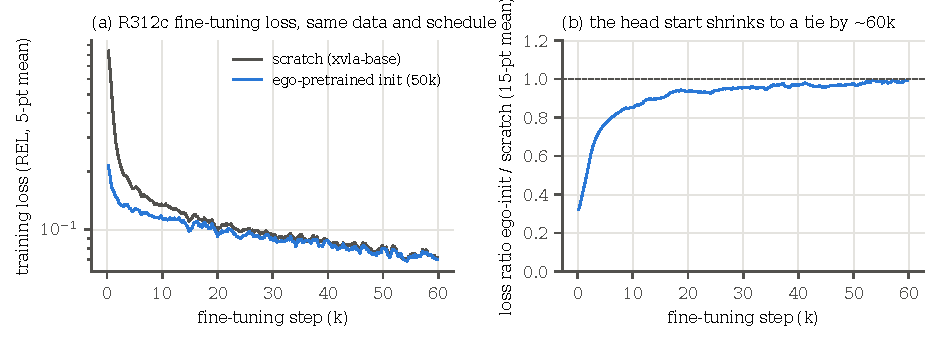
\includegraphics[width=\textwidth]{figures/fig5_ego_init_loss.pdf}
\caption{R312c fine-tuning from the base model versus from the 50k ego checkpoint, same data, schedule and seed. (a) Training
loss. (b) Ratio of the two; values below 1 favour the ego initialization. Training loss only.}
\label{fig:egoinit}
\end{figure*}

\textbf{Attempts to close the visual gap.} Applied to every frame (ROBOT100), the robot-like rendering of Sec.~\ref{sec:conv} drops the
wrist sharpness median from 1{,}854/1{,}487 to 181/132, still two to three times the robot's 59/64. A run with 70\% of frames
re-rendered was stopped at 5k steps; a co-training run with four ego (ROBOT100) and four robot samples per batch was stopped at 88.6k
steps without evaluation. A 300k ROBOT100 pretraining run (297 episodes, 48{,}411 rows, 49.6 epochs) finished on 5 October at a
training loss of 0.007; its checkpoints are the ego initializations of the next experiment. No offline transfer metric was computed
for the re-rendered models.

\textbf{Low-data ablation: 30 robot episodes.} The 312-episode comparison gives the robot data every chance to wash out the
initialization; the question that matters for using human data is whether it helps when robot data is scarce. We fine-tuned on R30
with R312c normalization statistics, seed 1000 and a 600k-step cosine schedule from three initializations: the base model
(scratch) and the ROBOT100 run at 100k and at 300k steps. The 100k checkpoint comes from the middle of the same 300k schedule, so its
learning rate had not decayed; it is not a separate 100k-step run. The arms ran on different machines (scratch and 100k-init on an
RTX~4090 with PyTorch~2.6, 300k-init on an RTX~5090 with PyTorch~2.7.1), so they are not bit-identical twins.

\begin{table}[t]
\centering\footnotesize\setlength{\tabcolsep}{4pt}
\caption{R30 fine-tuning, training loss (200-step running mean) at matched steps, and the ratio of window means to scratch
(below 1 favours the ego initialization). One seed per arm; no held-out or robot evaluation.}
\label{tab:r30}
\begin{tabular}{@{}lccc@{}}
\toprule
Step & Scratch & Ego-PT 100k init & Ego-PT 300k init \\
\midrule
200 & 0.801 & 0.239 & 0.446 \\
1k & 0.312 & 0.103 & 0.117 \\
10k & 0.065 & 0.056 & 0.040 \\
50k & 0.019 & 0.017 & 0.014 \\
100k & 0.009 & 0.009 & 0.007 \\
\midrule
Window & & ratio & ratio \\
\midrule
1k--5k & & 0.544 & 0.493 \\
10k--20k & & 0.823 & 0.697 \\
50k--100k & & 0.970 & 0.856 \\
100k--150k & & 1.021 & 0.914 \\
\bottomrule
\end{tabular}
\end{table}

Table~\ref{tab:r30} and Fig.~\ref{fig:r30} show the 312-episode pattern, stretched out. Both ego initializations start at less than
half the scratch loss (window ratio 0.54 and 0.49 over 1k--5k). The 100k-step initialization loses its advantage by about 100k steps
(ratio 0.97 over 50k--100k, 1.02 over 100k--150k); the 300k-step one keeps a smaller advantage longer (0.86 and 0.91) and reaches
parity at about 200k. Beyond about 150k all losses are 0.001--0.004 at the printed precision and ratios are not meaningful. The
100k-step initialization starts lower than the 300k-step one (0.239 versus 0.446 at step 200) although it was pretrained less; we
have not explained this. All three runs were stopped by us to free GPUs, at 471k, 305k and 310k, after 214, 139 and 141 epochs:
with 30 episodes every arm fits its training data almost exactly long before the schedule ends. Training loss here measures how fast
each initialization memorizes the robot data, not how well it acts; the relevant comparison is closed-loop at early and middle
checkpoints (roughly 10k--150k), and no R30 checkpoint has been run on the robot yet.

\begin{figure*}[t]
\centering
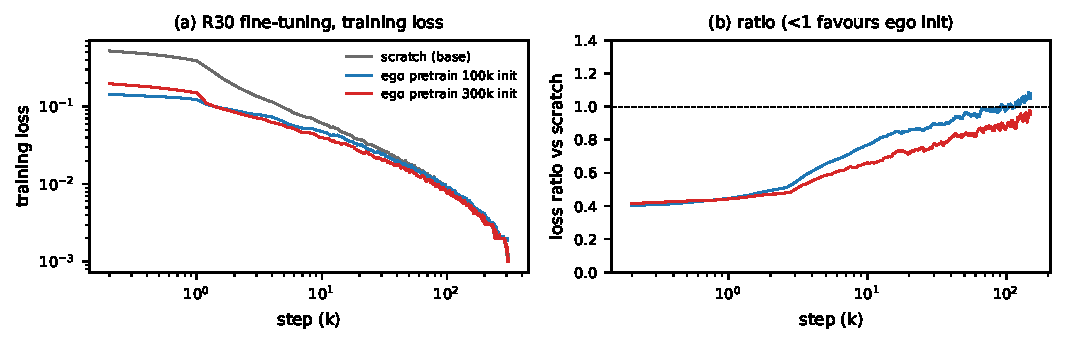
\includegraphics[width=0.8\textwidth]{figures/fig8_r30_ablation.pdf}
\caption{R30 fine-tuning (30 robot episodes) from the base model and from ego pretraining at 100k and 300k steps. (a) Training
loss (log--log, smoothed). (b) Ratio to scratch, shown to 150k; beyond that the 3-decimal losses make the ratio noise.
Training loss only, one seed per arm.}
\label{fig:r30}
\end{figure*}

\section{Results: Single-Arm Approach}\label{sec:res3}
Stacking showed that, once both domains share one action contract, the remaining gap is visual and geometric. A single-arm approach
to a cube isolates that gap with far fewer confounds: one arm, one object, no grasp, no task order, and success can be judged by eye.

\textbf{HRA\_red (v1).} Of 200 takes, 19 fail the cube-scale gates (14 with too few PnP frames, 5 with too large a spread) and 15 fail a
physical sanity check on the scaled trajectory (scale between 0.1 and 1.0, SLAM travel at least 0.8 of the PnP-observed approach
distance, travel at most 0.8\,m). The remaining 166 are split into 151 train episodes (20{,}319 rows) and 15 validation episodes
(2{,}011 rows); the median scale is 0.354 (p5 0.188, p95 0.500) and the median cube-centre residual 0.17\,cm. With the guessed-camera
rendering, the 300k-step run finished on 5 October at a training loss of 0.002 (118 epochs). Held-out loss rises from the first
evaluated checkpoint (Table~\ref{tab:val}, Fig.~\ref{fig:val}a): 0.150 at 15k (training subset 0.066), 0.198 at 30k, 0.213 at 60k,
0.265 at 90k and 0.299 at 105k, while the training-subset loss falls to 0.018. With 151 episodes the model overfits almost
immediately.

\begin{table}[t]
\centering\footnotesize\setlength{\tabcolsep}{3pt}
\caption{Single-arm held-out loss (masked MSE on the 9 supervised dimensions) by checkpoint; training-subset loss in parentheses.}
\label{tab:val}
\resizebox{\columnwidth}{!}{\begin{tabular}{@{}lccccc@{}}
\toprule
Dataset (val eps) & 5k & 15k & 30k & 45k/50k & 105k \\
\midrule
HRA\_red v1 (15) & -- & 0.150 (0.066) & 0.198 (0.053) & -- & 0.299 (0.018) \\
A100 A: start (11) & 0.124 (0.110) & 0.125 (0.058) & 0.141 (0.031) & 0.224 (0.020) & -- \\
A100 B: origin (11) & 0.132 (0.097) & 0.147 (0.057) & 0.174 (0.031) & 0.190 (0.022) & -- \\
\bottomrule
\end{tabular}}
\end{table}

\textbf{First robot runs and what they exposed.} v1 checkpoints from 15k to 75k ran 8{,}397 control cycles (658 run starts) on
4 October, and 100k, 200k and 300k ran 61 planned sessions on 6 October while the chunk-execution settings were tuned; the operator's
verdicts were ``accuracy dropped a lot'' and ``too much zigzag''. From a start near the cube the arm moved towards it; for cubes far
to the left it dragged along the table, by about 39 and 26\,cm in two runs. Interpreting these runs required knowing where the human
data sits relative to the robot, which v1 never did: its labels are relative motions of the UMI tool frame and its start state is the
human's own start. Linking takes to the robot base after the fact (cube in the head camera, wrist trajectory through cube PnP, tilt
from IMU gravity) linked only 64 of 166 takes, with start heights spread over 4\,cm and up-axis error p50 10\textdegree, p90
28\textdegree, and it exposed the 18\textdegree{} camera--IMU error of Sec.~\ref{sec:pose}. The human wrist camera at the take start
and the robot wrist camera at a reachable start cannot coincide: matching the human's view would need the shoulder joint past its
limit; the closest feasible start (pose A) puts the camera within 1--14\mm horizontally but 78\mm higher and 8\textdegree{} steeper.
Re-reading v1 200k from pose A with the jaw-tip model under three tool-frame conventions gave: tool axis unrotated, the tip ended
about 2\,cm from the cube and 3\,cm above the table; rotated by the 33.1\textdegree{} camera pitch, it overshot by about 11\,cm;
rotated and offset by the camera--TCP translation, it ended about 4\,cm from the cube and 10\,cm above the table. These are single
runs reconstructed from forward kinematics, not measurements of success. A run on robotcam v2 reached about 64k steps (training
loss 0.026) before being stopped.

\textbf{HRA\_A100: a shared origin.} Each take is an automatic cycle (Fig.~\ref{fig:protocol}): 5\,s rest; the operator places the
HandUMI jaw tip on the taped cross and holds it still for 2\,s; recording starts with a further 2\,s hold (the origin); a 3\,s ``ready''
phase moves the hand to a robot-like start pose; at ``go'' a 10\,s approach is recorded, and training data starts at ``go''. Cube
placements were planned as 40 centre, 20 left/right, 20 front/back and 20 edge. On 6 October 107 takes were kept in four sessions
(7, 8, 9 and 83 takes; the first session predates the origin hold). Scale comes from cube PnP or the origin plane, frame and yaw from
G (Secs.~\ref{sec:pose}--\ref{sec:conv}).

\begin{figure}[t]
\centering
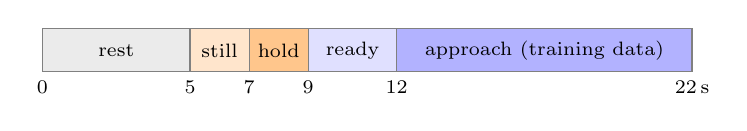
\begin{tikzpicture}[font=\scriptsize, x=0.375cm]
\foreach \a/\b/\t/\c in {0/5/rest/black!8, 5/7/still/orange!20, 7/9/hold/orange!45, 9/12/ready/blue!12, 12/22/approach (training data)/blue!30}
  {\fill[\c] (\a,0) rectangle (\b,0.55); \draw[black!50] (\a,0) rectangle (\b,0.55); \node at ({(\a+\b)/2},0.27) {\t};}
\foreach \x/\l in {0/0, 5/5, 7/7, 9/9, 12/12, 22/22\,s} \node[below] at (\x,0) {\l};
\end{tikzpicture}
\caption{HRA\_A100 take cycle: rest, jaw tip still on the taped cross, recording starts with a 2\,s origin hold, ready, 10\,s approach.
The origin hold places the HandUMI jaw tip on the same taped cross that the robot jaw tip touched during calibration.}
\label{fig:protocol}
\end{figure}

\textbf{Start-anchored versus origin-anchored state.} On 93 takes (82 train, 11 validation; the excluded 14 are the old session, 7
takes in which the hand moved over 20\mm during the hold, and one physics failure) we trained two otherwise identical models: A
anchors the state at the hand pose at ``go'', B at a fixed origin frame F (the cross, with the tape heading and the median hold
pitch). Both use robot-TCP labels and the robotcam v2 rendering. Their held-out losses are close and both are lowest at the first
checkpoint (Table~\ref{tab:val}, Fig.~\ref{fig:val}b): A 0.124 and B 0.132 at 5k, rising to 0.224 (A, 50k) and 0.190 (B, 45k). With 82
training takes, both overfit from 5k steps; neither anchoring is better on this measure.

\begin{figure*}[t]
\centering
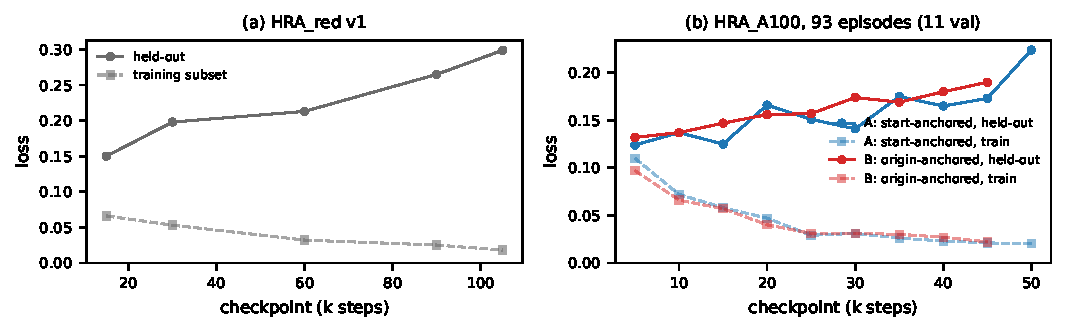
\includegraphics[width=0.8\textwidth]{figures/fig9_hra_val.pdf}
\caption{Held-out (solid) and training-subset (dashed) loss by checkpoint. (a) HRA\_red v1, 15 validation takes. (b) HRA\_A100,
start-anchored (A) and origin-anchored (B) state, 11 validation takes. All runs overfit from the earliest checkpoint.}
\label{fig:val}
\end{figure*}

\textbf{Start pose.} We compared ten candidate robot start poses derived from the median and medoid of the human ``go'' poses in G,
moved back, right and down; the operator preferred the lowest (pose 08, TCP $(273, -168, 116)$\mm, joint margin 9.1\textdegree). On
7 October 27 further takes were recorded with a lower human start (origin to ``go'' about 89\mm instead of about 247\mm); from pose 08
only 5 of them pass, so they were dropped, and the current run (CT7-old, 85 takes from 6 October, start 08, 100k-step schedule) uses
only the 6 October data. CT5 and CT6 runs were stopped after 7k and 3k steps while settings changed; there is no validation split
for CT6 and CT7.

\section{Deployment and Robot Observations}\label{sec:deploy}
\textbf{Inference and control.} The policy runs on a Mac (Apple-silicon GPU, bf16) with 5 (bimanual) or 10 (single arm) denoising
steps. The robot cameras are captured at 640$\times$480, resized to 224$\times$224 and normalized as in training; in single-arm mode
the left wrist image is black. The state follows the training contract (TCP poses from FK of the measured joints, relative to an
anchor taken at run start or to a fixed anchor file), and absolute targets $T_k=T_\text{now}A_k$ are solved by Pink~\cite{caron2024pink}
IK on the URDF. In \emph{PLAN mode} one forward pass is kept in flight and IK-solved rows (50.05\,ms apart) stream to the robot
service, which plays them as 100\,Hz knots in MIT impedance mode; a planned knot jumping more than 90\textdegree{} makes the arm hold.
Optional real-time chunking~\cite{black2025rtc} pulls each new chunk towards the previous chunk's not-yet-executed targets.

\textbf{Settings that mattered.} (i) \emph{Chunk execution}: successive 16-step chunks are blended. With an exponential blend of
0.25, no cross-fade, no smoothing and a minimum of one executed row per chunk, motion was acceptable; with the code defaults (0.35, 4
rows, 3\textdegree, 6 rows), which a restart of the interface silently restored on 7 October, the operator reported that
``inference quality had dropped a lot'' until the values were restored. Behaviour on the robot depends on settings that are not part
of the checkpoint; the loader now restores them. (ii) \emph{Tool-frame convention}: models trained on robot-TCP labels (robotcam v2,
A100) must run with zero camera pitch and zero camera--TCP offset; the 33.1\textdegree{} pitch and offset apply only to v1, and
anchored models must be served with the same anchor file (F for B, G for CT5--CT7). (iii) \emph{Cube-size stop}: after the arm was
seen pushing the cube instead of stopping, the interface measures the red cube's apparent size ($\sqrt{\text{area}}$ in pixels on the
raw 640$\times$480 wrist frame) every 0.1\,s and stops when two readings exceed a threshold (170--250\,px were used); in follow mode it
resumes when the cube shrinks below 85\% of the threshold. It is a proximity proxy, not verified contact. The wrist image was also
zoomed 1.5$\times$ because the cube looked smaller than in training at the same position. (iv) \emph{Guards}: during v1 the interface
stopped a run after 450\mm net travel, 80\mm between inferences, a still period, or an output above 250\mm or 60\textdegree; a 6\,s
limit ended runs after 1--4 cycles and was removed. For A100 models all numeric guards are off and the left arm and jaws stay locked.

\textbf{Stacking on the robot.} Gen-2 checkpoints were executed on the reBot through the deployment interface: 71 checkpoints,
49{,}431 control cycles and 1{,}681 run starts between 2 and 4 October. The cycle log records IK tracking of the model's own
waypoints, not task outcome, so it yields no success rate. Two operator observations were not logged. The ego-initialized model at
10k fine-tuning steps grasped cubes but picked the wrong colour. The ego-initialized model fine-tuned on R312c for 300k (B300,
checkpoints between 75k and 205k) completed the full three-cube stack in closed loop. The number of trials was not recorded and no
video was taken, so we state only that closed-loop three-cube stacking has been demonstrated, with no success rate. It also says
nothing about the value of ego pretraining: no scratch model trained on R312c was evaluated under the same protocol. Of the B300
checkpoints that stacked, only 150k and 200k survive a storage clean-up, so the demonstration can be re-run only from those. A trial
logger (checkpoint, robot data, instruction, layout, stack level 0--3, wrong colour, failure reason) was added on 4 October but has
not been used.

\textbf{Approach on the robot.} The planned-execution log records 192 sessions on 6 and 7 October. On 6 October, 65 sessions (v1
checkpoints, the chunk-setting tuning above) were all stopped by the operator except one, which the interface closed when a planned
row jumped by 90.9\textdegree. On 7 October, 127 sessions ran: B 45k (3), A 50k (6) and CT5 5k (4), then B 50k with the 1.5$\times$
zoom (114 sessions, many of them follow-mode resumes); 69 of the 127 ended on the cube-size stop and 58 were stopped by the operator.
The log has no outcome field, so we cannot say how many approaches reached the cube. The cube appears orange in the
fisheye-rendered training images and red on the robot camera, a colour gap we have not corrected.

\section{Corrections and Known Inconsistencies}\label{sec:corr}
Several of our own intermediate readings were wrong, each found by an independent check: the robot start tilt was 25\textdegree,
not 3\textdegree; the robot's wrist view is about 1.32$\times$ magnified and 11\textdegree{} lower than the human's, not 2.5$\times$;
``labels drive the tip 5\,cm into the table'' was the TCP--tip offset; the table height moved from $-54.3$ to $-5.9$ to $-27.1$\mm as
the contact model was fixed; IMU tilt statistics were off by up to 18\textdegree; a mean origin yaw caused false rejections; a
camera-orientation convention error in an earlier export corrupted rotations until a frame-regression test found it; and two of our
embodiment ids pointed at untrained soft prompts.

Writing this report also exposed inconsistencies in our code, which we list rather than hide. (1) An inter-arm clearance check is
used only in retargeting v2, not as a Gen-1 gate. (2) In the Gen-1 target code a binarized gripper label 1 means \emph{open},
although a comment says closed. (3) Three gripper calibrations are in use (Gen-1 ticks with a 67.5\mm aperture, the gcal1 caliper
knots for Gen-2, and the collector's open/closed files); each dataset names its own. (4) The camera--IMU time offsets used by the
exporter differ in sign and magnitude from the raw calibration output, and the conversion step is not recorded. (5) Two different
right fisheye calibration versions are used by the exporter and by one viewer tool. (6) The IK step thresholds are documented per
15\,Hz row but applied on 30\,fps rows. (7) In PLAN mode the bimanual path does not pass gripper widths to the waypoint solver, so
the jaws would likely stay closed; the single-arm runs, which hold the jaws, are unaffected. (8) Several diagnostics were run from
scripts outside the repository and their outputs are stored as captured logs, not re-run. (9) Fitting scripts for the G frame, the
fingertip box and the 18\textdegree{} camera--IMU correction are not in the repository; only their outputs are.

\section{Lessons}\label{sec:lessons}
Each of the following was found by an explicit check rather than by a loss curve. (i) \emph{Every pose or scale source has a regime
in which it fails silently}: ORB-SLAM3 across scene changes, MASt3R-SLAM on rare one-frame jumps, the IMU on slow motion, cube PnP on
oblique single-face views and the origin plane on a few takes (p90 error 37\%); only a second, independent reference shows the
failure. (ii) \emph{A pretrained model's conditioning interface has to be audited, not assumed}: two of our embodiment ids pointed at
soft prompts that had never been trained. (iii) \emph{When human and robot data share a tensor contract, the remaining gap can be
localized by swapping inputs between domains}; here it is the wrist images, not kinematics or normalization. (iv) \emph{A shared
physical origin is cheaper than post-hoc registration}: linking takes after the fact reached 64 of 166 with centimetre errors, while
a taped cross touched by both robot and human gives a common frame with a sub-millimetre line fit. (v) \emph{The TCP of the IK stack
is a convention, not the fingertip}; contact reasoning needs fingertip geometry. (vi) \emph{Training-loss comparisons of
initializations end in a tie whenever the robot data is fitted to near zero}, at 312 and at 30 episodes alike, and small single-task
sets overfit at once; only held-out or closed-loop evaluation at early checkpoints can show a benefit. (vii) \emph{Execution settings
are part of the policy}: blend and smoothing parameters that live in the interface changed robot behaviour more than a change of
checkpoint, and outcome logging has to exist before the robot runs, not after.

\section{Limitations and Future Work}\label{sec:lim}
\textbf{Stopped early, no conclusion:} the R90 fine-tuning comparison (two matched steps), the 70\%-re-rendered pretraining (5k
steps), the ego/robot co-training run (88.6k steps, never evaluated), the robotcam v2 run (64k) and the CT5/CT6 runs. \textbf{Not yet
done:} robot fine-tuning from the 996-segment checkpoints; any robot or held-out evaluation of the R30 arms; a held-out or closed-loop
comparison of ego-initialized and scratch models; outcome logging on the robot.

\textbf{Not supported by this study:} (i) a closed-loop success rate for stacking or approach, or any closed-loop difference between
ego-initialized and scratch models; (ii) generalization to new cube layouts, since layouts were not recorded and Gen-1 discards
absolute geometry by design; (iii) generalization to unseen stacking orders, since all six orders appear in training; (iv) transfer
beyond one operator, one scene and a few days; (v) any benefit of human data for robot learning beyond fitting the robot training
distribution faster; (vi) that the ego-only policy or the re-rendered wrist images transfer to robot cameras; (vii) colour grounding
in the approach data.

\textbf{Planned experiments:} log every robot trial (model, checkpoint, robot data size, start pose, layout, instruction, stack level
0--3 or reached yes/no, failure and stop reason) with fixed execution settings, and run 20--30 trials per model; compare scratch and
ego-initialized models at matched fine-tuning steps and at R30 for the step and data budget at which stacking first succeeds; test
early approach checkpoints (5k--15k) of A, B and CT7 from the same starts and cube positions; record layouts from the head camera and
hold out layout regions; hold out two orders entirely and test instruction following; correct the colour of rendered wrist images;
train with a static-phase-aware loss; and use the approach prior as the first segment of the stacking policy.

More broadly, this work is a first step towards egocentric human demonstrations as scalable supervision for robot policies: learning
human-to-robot representations that keep task geometry and intent while discarding embodiment detail, and evaluating them with
predictive world models before execution. The present results show that the bottleneck is as much in pose recovery, filtering,
calibration and evaluation design as in the policy.

\section{Conclusion}
We built an upstream open-source hand-worn gripper with an added wrist IMU, collected 349 bimanual stacking demonstrations and two
single-arm approach datasets, and turned them into robot training data in two ways. Retargeted to robot joints, the stacking data
teaches a 0.9B VLA the direction of held-out human motion (cosine 0.90 at $k{=}30$ on moving samples) but not the use of the order
instruction, and static-phase drift is hidden by aggregate metrics; multi-seed trajectory retrieval removes much of the retargeting
loss. Converted to the robot's own Cartesian contract, whole episodes survive without feasibility filters once silent SLAM jumps are
removed, and the remaining human-to-robot gap is visual and lies in the wrist images. As an initialization, ego pretraining speeds up
early robot fine-tuning at 312 and at 30 robot episodes, and the training-loss advantage disappears as the robot data is fitted. An
ego-initialized model has completed full three-cube stacks on the robot, so the task is solved in closed loop; whether ego pretraining
reaches that point with fewer robot episodes or steps is the open question. For slow single-arm motions, a known object and a shared
physical origin replace IMU scale and bring human data into the robot's frame with sub-centimetre consistency; models trained on
80--150 such takes overfit quickly and move towards the cube from nearby starts. Measured success rates, spatial and task-order
generalization, and a benefit on disjoint robot data require the controlled experiments listed above.

\appendices
\section{Code Map and Report History}\label{app:code}
\textbf{Code map} (paths in the repository): collector and protocols \code{collection/} (\code{autoloop.py}, \code{recorder.py},
\code{integrity.py}); hardware and IMU firmware \code{hardware/}, \code{collection/firmware/}; upstream licence, NOTICE and our patch
\code{upstream/}; export and sync \code{pipeline/export/}, \code{pipeline/census/}; MASt3R-SLAM wrapper and scales
\code{pipeline/mast3r_pose/}, \code{cart20/ego_cart20/cube_pnp.py}; Gen-1 \code{pipeline/pseudo_joint/}, \code{pipeline/retarget_v2/};
Gen-2 \code{cart20/} (contract, pose filter, converter, validators); single arm \code{hra/}; training \code{training/}; evaluation and
diagnostics \code{evaluation/}, \code{analysis/}; deployment \code{deploy/}; claim verification \code{analysis/verify_claims.py}.

\textbf{Report history.} Version 2 (30 September 2026) covered Gen-1 stacking; version 3 (4 October) added Gen-2 and transfer
diagnostics; version 4 (7 October) added the R30 ablation and split the work into Part I (stacking), Part II (approach) and a
methods document; version 4.1 (12 October) added the hardware description. This version 5 merges them into one report without
changing any result; the earlier documents remain in the repository.

\begin{thebibliography}{99}\footnotesize
\bibitem{chi2024umi} C.~Chi, Z.~Xu, C.~Pan, E.~Cousineau, B.~Burchfiel, S.~Feng, R.~Tedrake, and S.~Song, ``Universal manipulation interface: In-the-wild robot teaching without in-the-wild robots,'' in \emph{RSS}, 2024.
\bibitem{wang2024dexcap} C.~Wang, H.~Shi, W.~Wang, R.~Zhang, L.~Fei-Fei, and C.~K. Liu, ``DexCap: Scalable and portable mocap data collection system for dexterous manipulation,'' in \emph{RSS}, 2024.
\bibitem{ohkawa2026yubi} T.~Ohkawa, J.~Arima, Y.~Noguchi \emph{et al.}, ``YUBI: Yielding universal bidigital interface for bimanual dexterous manipulation at scale,'' arXiv:2606.10244, 2026.
\bibitem{handumi_hw} BrikHMP18 and HandUMI contributors, ``HandUMI: Hardware,'' GitHub repository, \url{https://github.com/murobotics-ai/handumi-hw} (first published as \texttt{robonet-ai/handumi-hw}), Apache-2.0, 2026. Commit \texttt{e58de33} used.
\bibitem{handumi_sw} BrikHMP18 and HandUMI contributors, ``HandUMI: Software,'' GitHub repository, \url{https://github.com/murobotics-ai/handumi-sw} (first published as \texttt{robonet-ai/handumi-sw}), Apache-2.0, 2026. Commit \texttt{33cc437} used.
\bibitem{kareer2024egomimic} S.~Kareer \emph{et al.}, ``EgoMimic: Scaling imitation learning via egocentric video,'' \emph{arXiv:2410.24221}, 2024.
\bibitem{wang2023mimicplay} C.~Wang \emph{et al.}, ``MimicPlay: Long-horizon imitation learning by watching human play,'' in \emph{CoRL}, 2023.
\bibitem{grauman2022ego4d} K.~Grauman \emph{et al.}, ``Ego4D: Around the world in 3,000 hours of egocentric video,'' in \emph{CVPR}, 2022.
\bibitem{zhao2023act} T.~Z. Zhao, V.~Kumar, S.~Levine, and C.~Finn, ``Learning fine-grained bimanual manipulation with low-cost hardware,'' in \emph{RSS}, 2023.
\bibitem{chi2023diffusion} C.~Chi, S.~Feng, Y.~Du, Z.~Xu, E.~Cousineau, B.~Burchfiel, and S.~Song, ``Diffusion policy: Visuomotor policy learning via action diffusion,'' in \emph{RSS}, 2023.
\bibitem{kim2024openvla} M.~J. Kim \emph{et al.}, ``OpenVLA: An open-source vision-language-action model,'' in \emph{CoRL}, 2024.
\bibitem{black2024pi0} K.~Black \emph{et al.}, ``$\pi_0$: A vision-language-action flow model for general robot control,'' \emph{arXiv:2410.24164}, 2024.
\bibitem{zheng2025xvla} J.~Zheng \emph{et al.}, ``X-VLA: Soft-prompted transformer as scalable cross-embodiment vision-language-action model,'' in \emph{ICLR}, 2026 (arXiv:2510.10274).
\bibitem{cadene2024lerobot} R.~Cadene \emph{et al.}, ``LeRobot: State-of-the-art machine learning for real-world robotics in PyTorch,'' \url{https://github.com/huggingface/lerobot}, 2024.
\bibitem{lipman2023flow} Y.~Lipman, R.~T.~Q. Chen, H.~Ben-Hamu, M.~Nickel, and M.~Le, ``Flow matching for generative modeling,'' in \emph{ICLR}, 2023.
\bibitem{murai2025mast3rslam} R.~Murai, E.~Dexheimer, and A.~J. Davison, ``MASt3R-SLAM: Real-time dense SLAM with 3D reconstruction priors,'' in \emph{CVPR}, 2025.
\bibitem{furgale2013kalibr} P.~Furgale, J.~Rehder, and R.~Siegwart, ``Unified temporal and spatial calibration for multi-sensor systems,'' in \emph{IROS}, 2013.
\bibitem{tsai1989handeye} R.~Y. Tsai and R.~K. Lenz, ``A new technique for fully autonomous and efficient 3D robotics hand/eye calibration,'' \emph{IEEE Trans. Robotics and Automation}, 1989.
\bibitem{xiao2024florence2} B.~Xiao \emph{et al.}, ``Florence-2: Advancing a unified representation for a variety of vision tasks,'' in \emph{CVPR}, 2024.
\bibitem{caron2024pink} S.~Caron \emph{et al.}, ``Pink: Python inverse kinematics based on Pinocchio,'' \url{https://github.com/stephane-caron/pink}, 2024.
\bibitem{black2025rtc} K.~Black, M.~Y. Galliker, and S.~Levine, ``Real-time execution of action chunking flow policies,'' \emph{arXiv:2506.07339}, 2025.
\end{thebibliography}
\end{document}
